\section{Annales.}  
%<–––––––––––––––––––––––––––––––––––––––––––––––––––––––––––––––––––––––––>
%                         Amérique du nord juin 2003
%<–––––––––––––––––––––––––––––––––––––––––––––––––––––––––––––––––––––––––>
\subsection{Amérique du nord juin 2003}

Soit le graphe G joint en annexe constitué des sommets A, B, C, D, E, F et G.

\begin{enumerate} 
\item Quel est son ordre et le degré de chacun de ses sommets ?
\item Reproduire sur la copie et compléter le tableau des distances entre deux sommets de G :

\medskip
\begin{center} 
\begin{tabular}{|l|c|c|c|c|c|c|c|}\hline
Distance    &    A  &   B   &   C   &   D   &   E   &   F   &   G   \\ \hline
A           &    X  &       &       &       &       &       &       \\ \hline
B           &    X  &   X   &       &       &       &       &       \\ \hline
C           &    X  &   X   &   X   &       &       &       &       \\ \hline
D           &    X  &   X   &   X   &   X   &       &       &       \\ \hline
E           &    X  &   X   &   X   &   X   &   X   &       &       \\ \hline
F           &    X  &   X   &   X   &   X   &   X   &   X   &       \\ \hline
G           &    X  &   X   &   X   &   X   &   X   &   X   &   X   \\ \hline
\end{tabular}
\end{center}

\medskip
En déduire le diamètre de ce graphe.
\item 
   \begin{enumerate} 
   \item Donner un sous-graphe complet d'ordre 3 de G.

Qu'en déduire pour le nombre chromatique de G ?
   \item Proposer une coloration du graphe G et en déduire son nombre chromatique.
   \end{enumerate}
\item Donner la matrice M associée à G (vous numéroterez les lignes et les  colonnes dans l'ordre alphabétique).
\item En utilisant la matrice $ M_2$ donnée en annexe 1, déduire le nombre de chaînes de longueur 2 partant de A sans y revenir.
\end{enumerate}

\medskip
\begin{minipage}[]{10cm}
\begin{tikzpicture}
    \Vertex[x=1.3,y=3.8]{A}
    \Vertex[x=4.2,y=5.5]{B}
    \Vertex[x=7.3,y=4]{C}
    \Vertex[x=8.5,y=1.5]{D}
    \Vertex[x=5,y=0]{E}
    \Vertex[x=3.6,y=4]{F}  
    \Vertex[x=0.7,y=1]{G}
    \Edges(A,B,C,D,E,G,A,F,E,C)
    \Edge(B)(F)
\end{tikzpicture}
\end{minipage}
\begin{minipage}[]{5cm}
M$^2 =
\begin{pmatrix}
    3   &   1   &   1   &   0   &   2   &   1   &   0\\
    1   &   3   &   0   &   1   &   2   &   1   &   1\\
    1   &   0   &   3   &   1   &   1   &   2   &   1\\
    0   &   1   &   1   &   2   &   1   &   1   &   1\\
    2   &   2   &   1   &   1   &   4   &   0   &   0\\
    1   &   1   &   2   &   1   &   0   &   3   &   2\\
    0   &   1   &   1   &   1   &   0   &   2   &   2\\
\end{pmatrix}$
\end{minipage}

\medskip
\begin{tkzexample}[code only]
\begin{tikzpicture}
    \Vertex[x=1.3,y=3.8]{A}     \Vertex[x=4.2,y=5.5]{B}
    \Vertex[x=7.3,y=4]{C}       \Vertex[x=8.5,y=1.5]{D}
    \Vertex[x=5,y=0]{E}         \Vertex[x=3.6,y=4]{F}
    \Vertex[x=0.7,y=1]{G}
    \Edges(A,B,C,D,E,G,A,F,E,C) \Edge(B)(F)
\end{tikzpicture}
\end{tkzexample}

%<–––––––––––––––––––––––––––––––––––––––––––––––––––––––––––––––––––––––––>
\vfill\newpage
%<–––––––––––––––––––––––––––––––––––––––––––––––––––––––––––––––––––––––––>
%                         Antilles-Guyane juin 2003
%<–––––––––––––––––––––––––––––––––––––––––––––––––––––––––––––––––––––––––>
\subsection{Antilles-Guyane juin 2003 }\label{ag03} 
%<–––––––––––––––––––––––––––––––––––––––––––––––––––––––––––––––––––––––––>
\begin{enumerate}
\item Un musée est constitué de 9 salles notées A, B, C, D, E, F, G, H et S.

Le plan du musée est représenté ci-dessous :

\medskip
\begin{center}
\begin{tikzpicture}
\draw (0,0) rectangle (8,6);
\draw(2,0)--(2,0.7);
\draw(2,1.3)--(2,2.7);
\draw(2,3.3)--(2,4.7);
\draw(2,5.3)--(2,6);
\draw(4,0)--(4,0.7);
\draw(4,1.3)--(4,2.7);
\draw(4,3.3)--(4,4.7);
\draw(4,5.3)--(4,6);
\draw(6,0)--(6,0.7);
\draw(6,1.3)--(6,2.7);
\draw(6,3.3)--(6,4.7);
\draw(6,5.3)--(6,6);
\draw(2,5.3)--(2,6);
\draw(4,5.3)--(4,6);
\draw(6,5.3)--(6,6);
\draw(2,2)--(2.7,2);
\draw(3.3,2)--(4.7,2);
\draw(5.3,2)--(6,2);
\draw(2,4)--(2.7,4);
\draw(3.3,4)--(4.7,4);
\draw(5.3,4)--(8,4);
\node at (1,3){S};
\node at (3,3){G};
\node at (3,1){D};
\node at (3,5){A};
\node at (5,1){H};
\node at (5,3){E};
\node at (5,5){B};
\node at (7,2){F};
\node at (7,5){C};
\end{tikzpicture}
\end{center}

\medskip
Ainsi, un visiteur qui se trouve dans la salle S peut atteindre directement les salles  A, B ou G. S'il se trouve dans la salle C, il peut se rendre directement dans la salle B, mais pas dans la salle F.

On s'intéresse au parcours d'un visiteur dans ce musée. On ne se préoccupe pas de la manière dont le visiteur accède au musée ni comment il en sort. Cette situation peut être modélisée par un graphe, les sommets étant les noms des salles, les arêtes représentant les portes de communication.

   \begin{enumerate} 
   \item Dessiner un graphe modélisant la situation décrite.
   \item Est-il possible de visiter le musée, en empruntant chaque porte une fois et une seule ?

Justifier en utilisant un théorème du cours sur les graphes.
\item Pour rompre une éventuelle monotonie, le conservateur du musée souhaite différencier chaque salle de sa ou des salles voisines (c'est-à-dire accessibles par une porte)  par la moquette posée au sol. Quel est le nombre minimum de types de moquettes nécessaires pour  répondre à ce souhait ? Justifier.
   \end{enumerate}
\item On note $M$ la matrice à 9 lignes et 9 colonnes associée au graphe précédent, en  convenant de l'ordre suivant des salles S, A, B, C, D, E, F, G, H. Le graphe n'étant pas orienté,  comment cela se traduit-il sur la matrice ?
\item  On donne la matrice :

\[M^4 = 
\begin{pmatrix}
18  &   12  &   11  &   02  &   20  &   12  & 06    & 12    & 12\\
12  &   20  &   03  &   06  &   11  &   20  & 05    & 18    & 05\\
11  &   03  &   16  &   00  &   19  &   03  & 08    & 04    & 12\\
02  &   06  &   00  &   03  &   01  &   07  & 01    & 04    & 01\\
20  &   11  &   19  &   01  &   31  &   09  & 11    & 12    & 19\\
12  &   20  &   03  &   07  &   09  &   28  & 09    & 20    & 09\\
06  &   05  &   08  &   01  &   11  &   09  & 09    & 08    & 09\\
12  &   18  &   04  &   04  &   12  &   20  & 08    & 20    & 06\\
12  &   05  &   12  &   01  &   19  &   09  & 09    & 06    & 17\\
\end{pmatrix}\]

   \begin{enumerate} 
   \item Combien y-a-t-il de chemins qui en 4 étapes, partent de D et reviennent à D ?
   \item Combien y-a-t-il de chemins qui en 4 étapes, partent de S et reviennent à C ? Les citer.
   \item Est-il toujours possible de joindre en 4 étapes deux salles quelconques ? Justifier.
   \end{enumerate}
\end{enumerate}

%<–––––––––––––––––––––––––––––––––––––––––––––––––––––––––––––––––––––––––>
\vfill\newpage
%<–––––––––––––––––––––––––––––––––––––––––––––––––––––––––––––––––––––––––>
Code du graphe précédent, uniquement fait avec tikz sans tkz-berge

\bigskip
\begin{tkzexample}[code only]
\begin{tikzpicture}
  \draw (0,0) rectangle (8,6);
  \draw(2,0)--(2,0.7);
  \draw(2,1.3)--(2,2.7);
  \draw(2,3.3)--(2,4.7);
  \draw(2,5.3)--(2,6);
  \draw(4,0)--(4,0.7);
  \draw(4,1.3)--(4,2.7);
  \draw(4,3.3)--(4,4.7);
  \draw(4,5.3)--(4,6);
  \draw(6,0)--(6,0.7);
  \draw(6,1.3)--(6,2.7);
  \draw(6,3.3)--(6,4.7);
  \draw(6,5.3)--(6,6);
  \draw(2,5.3)--(2,6);
  \draw(4,5.3)--(4,6);
  \draw(6,5.3)--(6,6);
  \draw(2,2)--(2.7,2);
  \draw(3.3,2)--(4.7,2);
  \draw(5.3,2)--(6,2);
  \draw(2,4)--(2.7,4);
  \draw(3.3,4)--(4.7,4);
  \draw(5.3,4)--(8,4);
  \node at (1,3){S};
  \node at (3,3){G};
  \node at (3,1){D};
  \node at (3,5){H};
  \node at (5,1){H};
  \node at (5,3){E};
  \node at (5,5){B};
  \node at (7,2){F};
  \node at (7,5){C};
\end{tikzpicture}
\end{tkzexample}


%<–––––––––––––––––––––––––––––––––––––––––––––––––––––––––––––––––––––––––>
\vfill\newpage
%<–––––––––––––––––––––––––––––––––––––––––––––––––––––––––––––––––––––––––>
%                         Asie juin 2003
%<–––––––––––––––––––––––––––––––––––––––––––––––––––––––––––––––––––––––––>
\subsection{Asie juin 2003 }\label{asj03} 
%<–––––––––––––––––––––––––––––––––––––––––––––––––––––––––––––––––––––––––>


\bigskip 
\begin{minipage}[l]{0,58\textwidth}
Dans la ville de GRAPHE, on s'intéresse aux principales rues permettant de relier différents lieux ouverts au public, à savoir la mairie (M), le centre commercial (C), la bibliothèque (B), la piscine (P) et le lycée (L). Chacun de ces lieux est désigné par son initiale. Le tableau ci-contre donne les rues existant entre ces lieux.
\end{minipage}\hfill
\begin{minipage}[]{0,38\textwidth}
\begin{center}
     \begin{tabular}{|*{5}{c|} c|} \cline{2-6}
        \multicolumn{1}{c|}{}
          & B   & C & L & M & P \\ \hline
        B &     & X &   & X & X \\ \hline
        C & X   &   & X & X &   \\ \hline
        L &     & X &   & X &   \\ \hline
        M & X   & X & X &   & X \\ \hline
        P & X   &   &   & X &   \\ \hline
    \end{tabular}
\end{center}
\end{minipage}

\medskip
\begin{enumerate} 
\item Dessiner un graphe représentant cette situation.
\item Montrer qu'il est possible de trouver un trajet empruntant une fois et une seule toutes les rues de ce plan. Justifier. Proposer un tel trajet.

Est-il possible d'avoir un trajet partant et arrivant du même lieu et passant une fois et une seule par toutes les rues ?


\begin{minipage}[b]{0,3\textwidth}
\item
 Dimitri habite dans cette ville ; le graphe ci-contre  donne le \textbf{nouveau} plan du quartier avec les sens de circulation dans les différentes rues et le temps de parcours entre les différents lieux.
\end{minipage}
\hspace{1cm}
 \begin{minipage}[c]{0,68\textwidth}
    \begin{tikzpicture}[>=latex]
      \SetGraphUnit{4}
      \tikzset{VertexStyle/.style  = {shape         = circle,
                                      draw          = black,
                                      inner sep     = 2pt,%
                                      minimum size  = 6mm,
                                      outer sep     = 0pt,
                                      fill          = gray!60}}
      \Vertex {P}
      \NOEA(P){B}
      \SOEA(P){M}
      \NOEA(B){D}
      \SOEA(B){C}
      \SOEA(C){L}
      \tikzset{LabelStyle/.style = {fill=white}}
      \tikzset{EdgeStyle/.style  = {<->}}
      \Edge[label=$4$](P)(M)
      \Edge[label=$9$](C)(M)
      \Edge[label=$4$](C)(L)
      \Edge[label=$5$](C)(D)
      \Edge[label=$10$](B)(M)
      \tikzset{EdgeStyle/.style  = {<->,bend right}}
      \Edge[label=$11$](L)(D)
      \tikzset{EdgeStyle/.style  = {->}}
      \Edge[label=$3$](C)(B)
      \Edge[label=$10$](D)(B)
      \Edge[label=$10$](L)(M)
      \Edge[label=$10$](B)(P)
    \end{tikzpicture}
  \end{minipage}
\end{enumerate}

%<–––––––––––––––––––––––––––––––––––––––––––––––––––––––––––––––––––––––––>
\vfill\newpage
%<–––––––––––––––––––––––––––––––––––––––––––––––––––––––––––––––––––––––––>
Code du graphe précédent

\bigskip
\begin{tkzexample}[code only]
\begin{minipage}[c]{0,68\textwidth}
\begin{tikzpicture}[>=latex]
    \SetGraphUnit{4}
    \tikzset{VertexStyle/.style  = {shape         = circle,
                                    draw          = black,
                                    inner sep     = 2pt,%
                                    minimum size  = 6mm,
                                    outer sep     = 0pt,
                                    fill          = gray!60}}
    \Vertex {P}
    \NOEA(P){B}
    \SOEA(P){M}
    \NOEA(B){D}
    \SOEA(B){C}
    \SOEA(C){L}
    \tikzset{LabelStyle/.style = {fill=white}}
    \tikzset{EdgeStyle/.style  = {<->}}
    \Edge[label=$4$](P)(M)
    \Edge[label=$9$](C)(M)
    \Edge[label=$4$](C)(L)
    \Edge[label=$5$](C)(D)
    \Edge[label=$10$](B)(M)
    \tikzset{EdgeStyle/.style  = {<->,bend right}}
    \Edge[label=$11$](L)(D)
    \tikzset{EdgeStyle/.style  = {->}}
    \Edge[label=$3$](C)(B)
    \Edge[label=$10$](D)(B)
    \Edge[label=$10$](L)(M)
    \Edge[label=$10$](B)(P)
\end{tikzpicture}
\end{minipage}
\end{tkzexample}

%<–––––––––––––––––––––––––––––––––––––––––––––––––––––––––––––––––––––––––>
\vfill\newpage
%<–––––––––––––––––––––––––––––––––––––––––––––––––––––––––––––––––––––––––>
%                         France juin 2003
%<–––––––––––––––––––––––––––––––––––––––––––––––––––––––––––––––––––––––––>
\subsection{France juin 2003 }\label{frj03} 
%<–––––––––––––––––––––––––––––––––––––––––––––––––––––––––––––––––––––––––>

Un concert de solidarité est organisé dans une grande salle de spectacle. À ce concert sont conviés sept artistes de renommée internationale Luther Allunison (A), John Biaise (B), Phil Colline (C), Bob Ditlâne (D), Jimi Endisque (E), Robert Fripe (F) et Rory Garaguerre (G).

Les différents musiciens invités refusant de jouer avec certains autres, l'organisateur du concert doit prévoir plusieurs parties de spectacle. Les arêtes du  graphe $\Gamma$ ci-dessous indiquent quels sont les musiciens qui refusent de jouer entre eux.

\medskip
\begin{center}
\begin{tikzpicture}
  \SetGraphUnit{4}
  \GraphInit[vstyle=Normal]
  \tikzset{EdgeStyle/.style = {line width = 2pt}}
  \tikzset{VertexStyle/.append style = {line width = 2pt}}
  \Vertex{D}
  \SOEA(D){E}
  \EA(E){F}
  \NOEA(F){G}
  \NOWE(G){A}
  \NOWE(A){B}
  \SOWE(B){C}
  \Edges(F,G,A,D,F,B,E,G,C,F,A,E,C,B)
\end{tikzpicture}
\end{center}

\medskip
\begin{enumerate} 
\item Déterminer la matrice associée au graphe $\Gamma$ (les sommets de $\Gamma$ étant classés dans l'ordre alphabétique).
\item Quelle est la nature du sous-graphe de $\Gamma '$ constitué des sommets A, E, F et G ?

Que peut-on en déduire pour le nombre chromatique $\chi(\Gamma)$ du graphe $\Gamma$ ?
\item Quel est le sommet de plus haut degré de $\Gamma$ ?

En déduire un encadrement de $\chi(\Gamma)$.
\item Après avoir classé l'ensemble des sommets de $\Gamma$ par ordre de degré décroissant, colorier le graphe $\Gamma$ figurant en annexe.
\item Combien de parties l'organisateur du concert doit-il  prévoir ?

Proposer une répartition des musiciens pour chacune de ces parties.
\end{enumerate}

\medskip

\begin{tkzexample}[code only]
\begin{tikzpicture}
  \SetGraphUnit{4}
  \GraphInit[vstyle=Normal]
  \tikzset{EdgeStyle/.style = {line width = 2pt}}
  \tikzset{VertexStyle/.append style = {line width = 2pt}}
  \Vertex{D}
  \SOEA(D){E}\EA(E){F}
  \NOEA(F){G}\NOWE(G){A}
  \NOWE(A){B}\SOWE(B){C}
  \Edges(F,G,A,D,F,B,E,G,C,F,A,E,C,B)
\end{tikzpicture}
\end{tkzexample}


%<–––––––––––––––––––––––––––––––––––––––––––––––––––––––––––––––––––––––––>
\vfill\newpage
%<–––––––––––––––––––––––––––––––––––––––––––––––––––––––––––––––––––––––––>
%                        CE juin 2003
%<–––––––––––––––––––––––––––––––––––––––––––––––––––––––––––––––––––––––––>
\subsection{Centres Étrangers juin 2003 }\label{cej03} 
%<–––––––––––––––––––––––––––––––––––––––––––––––––––––––––––––––––––––––––>

\bigskip
Un livreur d'une société de vente à domicile doit, dans son après-midi, charger son camion à l'entrepôt noté A, livrer cinq clients que nous noterons B, C, D, E et F, puis retourner à l'entrepôt. Le réseau routier, tenant compte des sens de circulation, et les temps de parcours (en minutes) sont indiqués sur le graphe G suivant :

\medskip
\begin{center}
  \begin{tikzpicture}[>=latex]
    \SetGraphUnit{4}
    \Vertex {F}
    \NOWE(F){A}
    \NOEA(F){B}
    \SOEA(F){C}
    \SOWE(F){D}
    \SOWE(A){E}
    \tikzstyle{EdgeStyle}=[->]
    \tikzstyle{LabelStyle}=[fill=white]
    \Edge[label=$4$](A)(E)
    \Edge[label=$4$](E)(D)
    \Edge[label=$9$](D)(A)
    \Edge[label=$2$](B)(A)
    \Edge[label=$11$](C)(B)
    \Edge[label=$3$](D)(F)
    \Edge[label=$6$](F)(A)
    \tikzstyle{EdgeStyle}=[->,bend left=15]
    \Edge[label=$2$](D)(C)
    \Edge[label=$2$](C)(D)
    \Edge[label=$3$](F)(B)
    \Edge[label=$3$](B)(F)
    \Edge[label=$6$](F)(C)
    \Edge[label=$6$](C)(F)
  \end{tikzpicture}
\end{center}

\begin{enumerate} 
\item Donner la matrice M associée au graphe G.

On utilisera le modèle suivant :

\begin{center}
    \begin{tabular}{|*{7}{c|}}\cline{2-7}
    \multicolumn{1}{c|}{}%
        & A & B & C & D & E & F \\ \hline
    A   &   &   &   &   &   &   \\ \hline
    B   &   &   &   &   &   &   \\ \hline
    C   &   &   &   &   &   &   \\ \hline
    D   &   &   &   &   &   &   \\ \hline
    E   &   &   &   &   &   &   \\ \hline
    F   &   &   &   &   &   &   \\ \hline
    \end{tabular}
\end{center}

\item  On donne la matrice M$^6$ :

\[\text{M}^6 = 
\begin{pmatrix}
    8   &   6   &   6   &   3   &   4   &   6 \\
    19  &   11  &   12  &   9   &   6   &   16\\
    36  &   28  &   23  &   22  &   18  &   34\\
    37  &   24  &   25  &   17  &   15  &   31\\
    15  &   12  &   9   &   10  &   8   &   15\\
    28  &   22  &   19  &   15  &   15  &   26\\
\end{pmatrix}\]

On s'intéresse aux chemins partant de l'entrepôt A et se terminant en A.

   \begin{enumerate} 
   \item Combien existe-t-il de chemins de longueur 6 reliant A à A ?
   \item Citer ces chemins.
   \item Parmi ceux qui passent par tous les sommets du graphe, lequel minimise le temps de parcours ?
   \item Quelle conséquence peut tirer le livreur du dernier résultat ?
   \end{enumerate}
\item Au départ de sa tournée, le livreur a choisi de suivre l'itinéraire le plus rapide. Malheureusement, le client C n'est pas présent au passage du livreur et celui-ci décide de terminer sa livraison par ce client. Indiquer  quel est le chemin le plus rapide pour revenir à l'entrepôt A à partir de C. La réponse devra être justifiée.
\end{enumerate}

%<–––––––––––––––––––––––––––––––––––––––––––––––––––––––––––––––––––––––––>
\vfill\newpage
%<–––––––––––––––––––––––––––––––––––––––––––––––––––––––––––––––––––––––––>
Code du graphe précédent

\bigskip
\begin{tkzexample}[code only]
\begin{tikzpicture}[>=latex]
  \SetGraphUnit{3}
  \Vertex {F}
  \NOWE(F){A}
  \NOEA(F){B}
  \SOEA(F){C}
  \SOWE(F){D}
  \SOWE(A){E}
  \tikzstyle{EdgeStyle}=[->]
  \tikzstyle{LabelStyle}=[fill=white]
  \Edge[label=$4$](A)(E)
  \Edge[label=$4$](E)(D)
  \Edge[label=$9$](D)(A)
  \Edge[label=$2$](B)(A)
  \Edge[label=$11$](C)(B)
  \Edge[label=$3$](D)(F)
  \Edge[label=$6$](F)(A)
  \tikzstyle{EdgeStyle}=[->,bend left=15]
  \Edge[label=$2$](D)(C)
  \Edge[label=$2$](C)(D)
  \Edge[label=$3$](F)(B)
  \Edge[label=$3$](B)(F)
  \Edge[label=$6$](F)(C)
  \Edge[label=$6$](C)(F)
\end{tikzpicture}
\end{tkzexample}
\vfill\newpage
%<–––––––––––––––––––––––––––––––––––––––––––––––––––––––––––––––––––––––––>
%<–––––––––––––––––––––––––––––––––––––––––––––––––––––––––––––––––––––––––>
%                         Amérique du Nord mai 2004
%<–––––––––––––––––––––––––––––––––––––––––––––––––––––––––––––––––––––––––>
\subsection{Amérique du Nord juin 2004 }\label{anm04} 
%<–––––––––––––––––––––––––––––––––––––––––––––––––––––––––––––––––––––––––>


\textbf{Les parties A et B sont indépendantes.}

\textbf{Partie A}

On considère le graphe G$_{1}$ ci-dessous :

\bigskip

\begin{center}
\begin{tikzpicture}[>=latex]
    \SetGraphUnit{6}
    \Vertex{F}%
    \NOEA(F){B}
    \SOEA(F){E}
    \EA(B){C}
    \EA(E){D}
    \NO(D){A}
    \Edges(B,F,E,D,A,E,B,A,F,B,C,F,D)
\end{tikzpicture}
\end{center}

\medskip

\begin{enumerate}
\item Justifier les affirmations suivantes :

A$_{1}$ : \og le graphe G$_1$ admet au moins une chaîne eulérienne \fg.

A$_{2}$ ; \og La chaîne DABCFBEFAE n'est pas une chaîne eulérienne de G$_1$ \fg.

\item Déterminer un sous-graphe complet de G$_1$, ayant le plus grand ordre possible. En déduire un minorant du nombre chromatique $\gamma$ de ce graphe.

\item Déterminer un majorant de ce nombre chromatique. (On justifiera la réponse).

\item En proposant une coloration du graphe G$_1$, déterminer son nombre chromatique.

\end{enumerate}

\medskip

\textbf{Partie B}

Soit la matrice M d'un graphe orienté G$_2$ dont les sommets A, B, C, D et E sont pris dans l'ordre alphabétique.

On donne \[
    M = 
\begin{pmatrix}
    0   &   1   &   1   &   1   &   0\\
    1   &   0   &   1   &   0   &   1\\
    1   &   1   &   0   &   0   &   1\\
    0   &   1   &   0   &   0   &   1\\
    1   &   1   &   0   &   1   &   0\\
\end{pmatrix}
\]
~et~
\[
    \text{M}^3 = 
\begin{pmatrix}
    6   &   6   &   4   &   5   &   3\\
    5   &   6   &   5   &   3   &   6\\
    5   &   7   &   4   &   3   &   6\\
    3   &   5   &   3   &   3   &   3\\
    6   &   6   &   3   &   3   &   5\\
\end{pmatrix}.
\]
\begin{enumerate}
\item Construire le graphe G$_2$.
\item Déterminer le nombre de chaînes de longueur 3 reliant B à D. Les citer toutes.
\end{enumerate}

%<–––––––––––––––––––––––––––––––––––––––––––––––––––––––––––––––––––––––––>
\vfill\newpage
%<–––––––––––––––––––––––––––––––––––––––––––––––––––––––––––––––––––––––––>
Code du graphe précédent

\bigskip
\begin{tkzexample}[code only]
\begin{tikzpicture}[>=latex]
  \SetGraphUnit{6}
  \Vertex{F}
  \NOEA(F){B}
  \SOEA(F){E}
  \EA(B){C}
  \EA(E){D}
  \NO(D){A}
  \Edges(B,F,E,D,A,E,B,A,F,B,C,F,D)
\end{tikzpicture}
\end{tkzexample}

%<–––––––––––––––––––––––––––––––––––––––––––––––––––––––––––––––––––––––––>
\vfill\newpage
%<–––––––––––––––––––––––––––––––––––––––––––––––––––––––––––––––––––––––––>
%                         CE mai 2004
%<–––––––––––––––––––––––––––––––––––––––––––––––––––––––––––––––––––––––––>
\subsection{Centres étrangers  mai 2004 }\label{cem04} 
%<–––––––––––––––––––––––––––––––––––––––––––––––––––––––––––––––––––––––––>

\bigskip
Un jardinier possède un terrain bien ensoleillé avec une partie plus ombragée.

Il décide d'y organiser des parcelles où il plantera 8 variétés de légumes :

\medskip
\begin{center}\begin{minipage}[t]{0.48\textwidth}
    \begin{itemize}
    \item de l'ail (A),
    \item des courges (Co),
    \item des choux (Ch),
    \item des poireaux (Px),
    \item des pois (Po),
    \item des pommes de terre (Pt),
    \item des radis (R),
    \item et des tomates (T).
    \end{itemize}
\end{minipage}\end{center}

\medskip
Il consulte un almanach où figurent des incompatibilités de plantes, données par les deux tableaux :

\medskip

\begin{minipage}[t]{0.46\textwidth}
\begin{tabular}{|l|l|}\hline
    \multicolumn{2}{|p{7cm}|}{Expositions incompatibles de plantes}\\
\hline
    \multicolumn{1}{|p{3.5cm}|}{Plantes d'ombre partielle}
    &\multicolumn{1}{|p{3.5cm}|}{Plantes de plein soleil}\\ 
\hline
    &                       \\
    &   choux               \\
        pois    &   tomates \\
        radis   &   courges \\
    &                       \\
    &                       \\ 
\hline
    \multicolumn{2}{|p{7cm}|}{Par exemple : les pois sont incompatibles avec les
    choux, les tomates et les courges}\\ \hline
\end{tabular}
\end{minipage}
\hfill
\raisebox{6pt}{\begin{minipage}[t]{0.46\textwidth}
\begin{tabular}{|l|l|}\hline
\multicolumn{2}{|p{7cm}|}{Associations incompatibles de} \\
\multicolumn{2}{|p{7cm}|}{plantes dans une même parcelle}\\ \hline
 pois & ail, poireaux\\ \hline
pommes de & courges, radis et\\
terre & tomates\\ \hline
& tomates, ail\\
choux & poireaux et courges\\ \hline
courges & tomates\\ \hline
\multicolumn{2}{|p{7cm}|}{Par exemple : les pois sont incompatibles avec
l'ail et les poireaux}\\ \hline
\end{tabular}
\end{minipage}}

\medskip

Pour tenir compte de ces incompatibilités le jardinier décide de modéliser la situation sous la forme d'un graphe de huit sommets, chaque sommet représentant un légume.
\medskip
\begin{enumerate}
\item Sur la feuille annexe : compléter le graphe mettant en évidence les incompatibilités d'exposition ou les associations incompatibles indiquées dans les deux tableaux ci-dessus.

\item Calculer la somme des degrés des sommets du graphe, en déduire le nombre de ses arêtes.

\item Rechercher un sous-graphe complet d'ordre 4, qu'en déduit-on pour le nombre chromatique du graphe ?

\item Donner le nombre chromatique du graphe et l'interpréter en nombre minimum de parcelles que le jardinier devra créer.

\item Donner une répartition des plantes pur parcelle de façon à ce que chaque parcelle contienne exactement deux types de plantes et que le nombre de parcelles soit minimum.

\item Donner une répartition des plantes de façon à ce qu'une parcelle contienne trois plantes et que le nombre de parcelles soit minimum.
\end{enumerate}

\medskip
\begin{center}
  \begin{tikzpicture}
     \tikzstyle{VertexStyle}= [shape       = circle,
                               fill         = white,%
                               minimum size = 26pt,%
                               draw]
      \Vertex[x=1,y=0.8]{R}
      \Vertex[x=0.2,y=3.3]{Po}
      \Vertex[x=0,y=2]{Pt}
      \Vertex[x=0.9,y=5]{Px}
      \Vertex[x=3.5,y=5]{A}
      \Vertex[x=5.6,y=3.4]{T}
      \Vertex[x=5.3,y=2]{Co}
      \Vertex[x=3.3,y=0.2]{Ch}
      \Edges(Po,Px,Po,A,Po,T,Po,Co,Po,Ch)
    \end{tikzpicture}
\end{center}

%<–––––––––––––––––––––––––––––––––––––––––––––––––––––––––––––––––––––––––>
\vfill\newpage
%<–––––––––––––––––––––––––––––––––––––––––––––––––––––––––––––––––––––––––>
Code du graphe précédent

\bigskip
\begin{tkzexample}[code only]
\begin{tikzpicture}
 \tikzstyle{VertexStyle}= [shape       = circle,
                           fill         = white,%
                           minimum size = 26pt,%
                           draw]
  \Vertex[x=1,y=0.8]{R}
  \Vertex[x=0.2,y=3.3]{Po}
  \Vertex[x=0,y=2]{Pt}
  \Vertex[x=0.9,y=5]{Px}
  \Vertex[x=3.5,y=5]{A}
  \Vertex[x=5.6,y=3.4]{T}
  \Vertex[x=5.3,y=2]{Co}
  \Vertex[x=3.3,y=0.2]{Ch}
  \Edges(Po,Px,Po,A,Po,T,Po,Co,Po,Ch)
\end{tikzpicture}
\end{tkzexample}

%<–––––––––––––––––––––––––––––––––––––––––––––––––––––––––––––––––––––––––>
\vfill\newpage
%<–––––––––––––––––––––––––––––––––––––––––––––––––––––––––––––––––––––––––>
%                         France mai 2004
%<–––––––––––––––––––––––––––––––––––––––––––––––––––––––––––––––––––––––––>
\subsection{France  juin 2004}
%<–––––––––––––––––––––––––––––––––––––––––––––––––––––––––––––––––––––––––>

Le graphe ci-dessous indique, sans respecter d'échelle, les parcours possibles entre les sept bâtiments d'une entreprise importante.

\medskip
\begin{tikzpicture}
  \SetGraphUnit{5}
  \Vertex{A}
  \NOEA(F){B}
  \SOEA(F){E}
  \EA(B){C}
  \EA(E){D}
  \NO(D){A}
  \Edges(F,E,F,D,F,C,F,A,F,B,A,E,E,D,D,A,B,A,C,B,E,B)
\end{tikzpicture}

Un agent de sécurité effectue régulièrement des rondes de surveillance. Ses temps de parcours en minutes entre deux bâtiments sont les
suivants :

\medskip
\begin{center}
\begin{minipage}{0.5\textwidth}
    \begin{itemize}
    \item AB : 16 minutes ;
    \item AG : 12 minutes ;
    \item BC : 8 minutes ;
    \item BE : 12 minutes ;
    \item BG : 8 minutes ;
    \item CD : 7 minutes ;
    \item CE : 4 minutes ;
    \item CG : 10 minutes ;
    \item DE : 2 minutes ;
    \item EF : 8 minutes ;
    \item EG : 15 minutes ;
    \item FG : 8 minutes.
    \end{itemize}
\end{minipage}
\end{center}

\medskip
Sur chaque arête, les temps de parcours sont indépendants du sens de parcours.

\begin{enumerate}
\item En justifiant la réponse, montrer qu'il est possible que l'agent de sécurité passe une fois et une seule par tous les chemins de cette usine. Donner un exemple de trajet.

\item L'agent de sécurité peut-il revenir à son point de départ après avoir parcouru une fois et une seule tous les chemins ? Justifier la réponse.

\item Tous les matins, l'agent de sécurité part du bâtiment A et se rend au bâtiment D.

En utilisant un algorithme que l'on explicitera, déterminer le chemin qu'il doit suivre pour que son temps de parcours soit le plus court possible, et donner ce temps de parcours.
\end{enumerate}

\medskip
\begin{tkzexample}[code only]
\begin{tikzpicture}
   \SetGraphUnit{5}
    \Vertex{A}   \NOEA(F){B}  \SOEA(F){E}
    \EA(B){C}    \EA(E){D}    \NO(D){A}
    \Edges(F,E,F,D,F,C,F,A,F,B,A,E,E,D,D,A,B,A,C,B,E,B)
\end{tikzpicture}
\end{tkzexample}
%<–––––––––––––––––––––––––––––––––––––––––––––––––––––––––––––––––––––––––>
\vfill\newpage
%<–––––––––––––––––––––––––––––––––––––––––––––––––––––––––––––––––––––––––>

%<–––––––––––––––––––––––––––––––––––––––––––––––––––––––––––––––––––––––––>
%                         La Reunion mai 2004
%<–––––––––––––––––––––––––––––––––––––––––––––––––––––––––––––––––––––––––>
\subsection{La Réunion juin 2004 }\label{larj04} 
%<–––––––––––––––––––––––––––––––––––––––––––––––––––––––––––––––––––––––––>


\textbf{Partie A}

On note $G$ le graphe représenté ci-dessous et $M$ sa matrice obtenue en prenant les sommets dans l'ordre alphabétique. La matrice $M^3$ est également donnée.

\medskip
\begin{center}
\begin{tikzpicture}[>=latex]
    \SetGraphUnit{4.5}
    \Vertex {e}
    \NOEA(e){f}
    \SOEA(e){d}
    \SOEA(f){h}
    \Vertex[position={above of=e,yshift=2cm}]{g}
    \Vertex[position={left  of=g,xshift=-1cm}]{c} 
    \Vertex[position={left  of=d,xshift=-2cm}]{a} 
    \SOWE(c){b}
    \Edges(a,c,g)  \Edges(d,h,f,e,d,a,e,g,a,b,c,e)
    \Edge[style={bend left}](g)(h)
\end{tikzpicture}
\end{center}

\bigskip
\begin{center}
 $M^3 = \begin{pmatrix}
    10  &   8   &   11  &   10  &   12  &   5   &   13  &   4\\
    8   &   2   &   7   &   3   &   5   &   2   &   4   &   3\\
    11  &   7   &   8   &   6   &   12  &   3   &   10  &   5\\
    10  &   3   &   6   &   2   &   11  &   1   &   4   &   8\\
    12  &   5   &   12  &   11  &   8   &   8   &   13  &   3\\
    5   &   2   &   3   &   1   &   8   &   0   &   2   &   6\\
    13  &   4   &   10  &   4   &   13  &   2   &   6   &   9\\
    4   &   3   &   5   &   8   &   3   &   6   &   9   &   0\\
\end{pmatrix}$
\end{center}


\bigskip
Dire, en justifiant votre réponse, si les affirmations suivantes sont vraies ou
 fausses :

\begin{enumerate}
\item L'ordre du graphe est égal au plus grand des degrés des sommets.
\item Le graphe $G$ contient un sous-graphe complet d'ordre $3$.
\item Les sommets de $G$ peuvent être coloriés avec trois couleurs sans que deux sommets adjacents soient de même couleur.
\item Il est possible de parcourir ce graphe en passant une fois et une seule par chaque arête.
\item Il existe au moins un chemin de longueur $3$ qui relie chaque sommet à chacun  des sept autres sommets du graphe.
\item il y a $72$ chemins de longueur $3$ qui relient le sommet $e$ à chacun des huit sommets du graphe.
\end{enumerate}

\newpage

\textbf{ Partie B}

Le graphe suivant représente un réseau de lignes d'autobus. Les sommets du graphe désignent les arrêts. Les poids des arêtes sont les durées de parcours,  en minutes, entre deux arrêts (correspondances comprises).

\medskip
\begin{center}
\begin{tikzpicture}[>=latex]
      \SetGraphUnit{4.5}
    \Vertex {e}
    \NOEA(e){f}
    \SOEA(e){d}
    \SOEA(f){h}
    \Vertex[position={above  of=e,yshift=2cm}]{g}
    \Vertex[position={left  of=g,xshift=-1cm}]{c}
    \Vertex[position={left  of=d,xshift=-2cm}]{a}
    \SOWE(c){b}
    \tikzstyle{LabelStyle}=[fill=white]
    \Edge[label=$3$](a)(b)
    \Edge[label=$11$](a)(c)
    \Edge[label=$6$](a)(e)
    \Edge[label=$17$](a)(d)
    \Edge[style={pos=.25},label=$20$](a)(g)
    \Edge[label=$5$](c)(b)
    \Edge[label=$6$](c)(e)
    \Edge[label=$7$](c)(g)
    \Edge[label=$7$](f)(e)
    \Edge[label=$3$](d)(e)
    \Edge[label=$9$](d)(h)
    \Edge[label=$6$](g)(e)
    \Edge[style={bend left},label=$11$](g)(h)
    \Edge[label=$4$](f)(h)
\end{tikzpicture}
\end{center}

\medskip
Déterminer, à l'aide d'un algorithme, la durée minimum pour aller de l'arrêt $a$  à l'arrêt $h$ et donner ce trajet.
%<–––––––––––––––––––––––––––––––––––––––––––––––––––––––––––––––––––––––––>
\vfill\newpage
%<–––––––––––––––––––––––––––––––––––––––––––––––––––––––––––––––––––––––––>
Code du graphe précédent

\medskip
\begin{tkzexample}[code only]
\begin{tikzpicture}[>=latex]
    \SetGraphUnit{4.5}
    \Vertex {e}
    \NOEA(e){f}
    \SOEA(e){d}
    \SOEA(f){h}
    \Vertex[position={above of=e,yshift=2cm}]{g}
    \Vertex[position={left  of=g,xshift=-1cm}]{c} 
    \Vertex[position={left  of=d,xshift=-2cm}]{a} 
    \SOWE(c){b}
    \Edges(a,c,g)  \Edges(d,h,f,e,d,a,e,g,a,b,c,e)
    \Edge[style={bend left}](g)(h)
\end{tikzpicture}
\end{tkzexample}

et

\begin{tkzexample}[code only]
\begin{tikzpicture}[>=latex]
    \SetGraphUnit{4.5}
    \Vertex {e}
    \NOEA(e){f}
    \SOEA(e){d}
    \SOEA(f){h}
    \Vertex[position={above  of=e,yshift=2cm}]{g}
    \Vertex[position={left  of=g,xshift=-1cm}]{c}
    \Vertex[position={left  of=d,xshift=-2cm}]{a}
    \SOWE(c){b}
    \tikzstyle{LabelStyle}=[fill=white]
    \Edge[label=$3$](a)(b)
    \Edge[label=$11$](a)(c)
    \Edge[label=$6$](a)(e)
    \Edge[label=$17$](a)(d)
    \Edge[style={pos=.25},label=$20$](a)(g)
    \Edge[label=$5$](c)(b)
    \Edge[label=$6$](c)(e)
    \Edge[label=$7$](c)(g)
    \Edge[label=$7$](f)(e)
    \Edge[label=$3$](d)(e)
    \Edge[label=$9$](d)(h)
    \Edge[label=$6$](g)(e)
    \Edge[style={bend left},label=$11$](g)(h)
    \Edge[label=$4$](f)(h)
\end{tikzpicture}
\end{tkzexample}

%<–––––––––––––––––––––––––––––––––––––––––––––––––––––––––––––––––––––––––>
\vfill\newpage
%<–––––––––––––––––––––––––––––––––––––––––––––––––––––––––––––––––––––––––>
\subsection{Amérique du Sud Nov 2006}\label{amsn06} 
\begin{enumerate}
\item À l'occasion de la coupe du monde de football 2006 en Allemagne, une agence touristique organise des voyages en car à travers les différentes villes où se joueront les matchs d'une équipe nationale.

Les routes empruntées par les cars sont représentées par le graphe ci-dessous. Le long de chaque arête figure la distance en kilomètres séparant les villes.
Les lettres B, D, F, H, K, M, N et S représentent les villes Berlin, Dortmnd, Francfort, Hambourg, Kaiserslautern, Munich, Nuremberg et Stuttgart.

\bigskip

\begin{center}
\begin{tikzpicture}
  \Vertex[x=0 ,y=0]{K}
  \Vertex[x=0 ,y=2]{F}
  \Vertex[x=-1,y=4]{D}
  \Vertex[x=3 ,y=7]{H}
  \Vertex[x=8 ,y=5]{B}
  \Vertex[x=9 ,y=2]{N}
  \Vertex[x=5 ,y=0]{M}
  \Vertex[x=3 ,y=1]{S}
  \tikzstyle{LabelStyle}=[fill=white,sloped]
  \tikzstyle{EdgeStyle}=[bend left]
  \Edge[label=$120$](K)(F)
  \Edge[label=$650$](H)(S)
  \Edge[label=$780$](H)(M) 
  \Edge[label=$490$](D)(B) 
  \Edge[label=$600$](D)(M)
  \Edge[label=$580$](B)(M)
  \Edge[label=$600$](H)(N)
  \Edge[label=$490$](F)(H)
  \tikzstyle{EdgeStyle}=[bend right]
  \Edge[label=$630$](S)(B)
  \Edge[label=$210$](S)(N) 
  \Edge[label=$230$](S)(M) 
\end{tikzpicture}
\end{center}

\bigskip
En précisant la méthode utilisée, déterminer le plus court chemin possible pour aller de Kaiserslautern à Berlin en utilisant les cars de cette agence.
\item Pour des raisons de sécurité, les supporters de certaines équipes nationales participant à la coupe du monde de football en 2006 ne peuvent être logés dans le même hôtel.

On donne ci-dessous le graphe d'incompatibilité entre les supporters de différentes équipes : par exemple, un supporter de l'équipe A ne peut être logé avec un supporter de l'équipe P.

\bigskip
\begin{center}
\begin{tikzpicture}
 \tikzstyle{EdgeStyle}=[bend left]
 \Vertex[x=0,y=0]{G}
 \Vertex[x=0,y=3]{A} 
 \Vertex[x=3,y=5]{P}
 \Vertex[x=4,y=2]{C}
 \Vertex[x=8,y=3]{Q}
 \Vertex[x=7,y=0]{E}
 \Vertex[x=3,y=-1]{R}
 \Edges(G,A,P,Q,E) \Edges(C,A,Q) \Edges(C,R,G) \Edges(P,E,A)
\end{tikzpicture}
\end{center}

\bigskip
\begin{enumerate}
\item  Déterminer le nombre chromatique de ce graphe en justifiant la valeur trouvée. 
\item  Proposer une répartition des supporters par hôtel en utilisant un nombre minimum d'hôtels.
\end{enumerate}
\end{enumerate}
%<–––––––––––––––––––––––––––––––––––––––––––––––––––––––––––––––––––––––––>
\vfill\newpage\null 
%<–––––––––––––––––––––––––––––––––––––––––––––––––––––––––––––––––––––––––>
%                        Liban juin 2006
%<–––––––––––––––––––––––––––––––––––––––––––––––––––––––––––––––––––––––––>
\subsection{Liban juin 2006 }\label{lib06} 
%<–––––––––––––––––––––––––––––––––––––––––––––––––––––––––––––––––––––––––>

\begin{enumerate}
\item  Dans un parc, il y a cinq bancs reliés entre eux par des allées.

On modélise les bancs par les sommets A, B, C, D, E et les allées par les arêtes du
graphe G ci-dessous :


\medskip
\begin{center}
\begin{tikzpicture}
     \SetGraphUnit{3} 
    \tikzstyle{VertexStyle}=[shape        = circle,
                             fill         = black,
                             minimum size = 20pt,
                             text         = white,
                             draw]   
    \Vertex[L= {\textbf{E}}]{E}
    \NOEA[L  = {\textbf{A}}](E){A}
    \SOEA[L  = {\textbf{D}}](E){D}
    \EA[L    = {\textbf{C}}](D){C}
    \NOEA[L  = {\textbf{B}}](C){B}  
   \tikzstyle{EdgeStyle}=[double           = orange,%
                          double distance  = 1pt,%
                          thick,%
                          bend right       = 20]
    \Edges(B,A,E,D,C,B,D)
\end{tikzpicture}
\end{center}

\medskip

\begin{enumerate}
\item On désire peindre les bancs de façon que deux bancs reliés par une allée soient
toujours de couleurs différentes.

Donner un encadrement du nombre minimal de couleurs nécessaires et justifier.

Déterminer ce nombre.
\item Est-il possible de parcourir toutes les allées de ce parc sans passer deux fois par
la même allée?
\end{enumerate}
\item Une exposition est organisée dans le parc. La fréquentation devenant trop importante, on décide d'instaurer un plan de circulation : certaines allées deviennent à sens unique, d'autres restent à double sens. Par exemple la circulation dans l'allée
située entre les bancs B et C pourra se faire de B vers C et de C vers B, alors que la circulation dans l'allée située entre les bancs A et B ne pourra se faire que de A vers B. Le graphe G$'$ ci-dessous modélise cette nouvelle situation :

\medskip
\begin{center}
\begin{tikzpicture}
     \SetGraphUnit{3} 
    \tikzstyle{VertexStyle}=[shape        = circle,
                             fill         = black,
                             minimum size = 20pt,
                             text         = white,
                             draw]   
    \tikzstyle{TempStyle}=[double           = orange,%
                           double distance  = 1pt]
    \Vertex[L= {\textbf{E}}]{E}
    \NOEA[L  = {\textbf{A}}](E){A}
    \SOEA[L  = {\textbf{D}}](E){D}
    \EA[L    = {\textbf{C}}](D){C}
    \NOEA[L  = {\textbf{B}}](C){B}  
    \tikzstyle{EdgeStyle}=[TempStyle,%
                           post,%
                           bend right      = 20]
    \Edges(A,E,D,C,B,D)
    \tikzstyle{EdgeStyle}=[TempStyle,%
                           pre,%
                           bend right      = 20]
    \Edges(B,A) 
    \tikzstyle{EdgeStyle}=[TempStyle,%
                           pre,%
                           bend left       = 20]
    \Edges(A,E,D,C,B)
\end{tikzpicture}
\end{center}

\begin{enumerate}
\item Donner la matrice M associée au graphe G$'$. (On ordonnera les sommets
par ordre alphabétique).
\item On donne M$^5
= \begin{pmatrix}
1& 6& 9& 6& 10\\
4& 5& 7& 11& 5\\
4& 6& 6& 11& 5\\
1& 5& 10& 6& 10\\
6& 5& 5& 14& 2\\
\end{pmatrix}$

Combien y a-t-il de chemins de longueur 5 permettant de se rendre du
sommet D au sommet B ?

Les donner tous.
\item Montrer qu'il existe un seul cycle de longueur 5 passant par le sommet A.

Quel est ce cycle ?

En est-il de même pour le sommet B ?
 \end{enumerate}
\end{enumerate}

\vfill\newpage\null
Code des graphes précédents

\begin{tkzexample}[code only]
\begin{tikzpicture}
   \SetGraphUnit{3} 
   \tikzstyle{VertexStyle}=[shape        = circle,
                            fill         = black,
                            minimum size = 20pt,
                            text         = white,
                            draw]
   \Vertex[L= {\textbf{E}}]{E}
   \NOEA[L  = {\textbf{A}}](E){A}
   \SOEA[L  = {\textbf{D}}](E){D}
   \EA[L    = {\textbf{C}}](D){C}
   \NOEA[L  = {\textbf{B}}](C){B} 
   \tikzstyle{EdgeStyle}=[double           = orange,
                          double distance  = 1pt,
                          thick,
                          bend right       = 20]
    \Edges(B,A,E,D,C,B,D)
\end{tikzpicture}
\end{tkzexample}

\begin{tkzexample}[code only]
\begin{tikzpicture}
     \SetGraphUnit{3} 
    \tikzstyle{VertexStyle}=[shape        = circle,
                             fill         = black,
                             minimum size = 20pt,
                             text         = white,
                             draw]
    \tikzstyle{TempStyle}=[double           = orange,
                           double distance  = 1pt]
    \Vertex[L= {\textbf{E}}]{E}
    \NOEA[L  = {\textbf{A}}](E){A}
    \SOEA[L  = {\textbf{D}}](E){D}
    \EA[L    = {\textbf{C}}](D){C}
    \NOEA[L  = {\textbf{B}}](C){B}
    \tikzstyle{EdgeStyle}=[TempStyle,
                           post,
                           bend right      = 20]
    \Edges(A,E,D,C,B,D)
    \tikzstyle{EdgeStyle}=[TempStyle,%
                           pre,%
                           bend right      = 20]
    \Edges(B,A) 
    \tikzstyle{EdgeStyle}=[TempStyle,%
                           pre,%
                           bend left       = 20]
    \Edges(A,E,D,C,B)
\end{tikzpicture}
\end{tkzexample}

\endinput